% ---------------------------------------------------------------------------
% CHAPTER 5 (RQ2). Rewritten in November 2026 with AI assistance (Claude) from
% Package H of the review docs/thesis/reviews/2026-11-15-g-focus-length-voice.md
% (results.json, part ch5: drafts, rewrites, actions C5-06 to C5-23), every
% fix of its verification (verify.json) that concerns this chapter, and the
% author's decisions: the owner and the loop defined in the opening; the
% changes of PR #181 listed there once; Storage folded into 5.2 and 5.5; one
% screenshot in Figure 5.2; Table 5.2 in two columns; the floor of five set
% against the four sources the author read; the answer halved. The engine is
% described, and the study run, at 2e146f51; the event log and the
% detectors are the same at the pin \thesisCommit. Every removed passage is kept verbatim in the defence notes.
% Open: Figure 5.1 (figures/src/f23-loop.tex) still carries three labels that
% the text contradicts (action C5-19).
% The author must read, revise and own every sentence before submission.
% ---------------------------------------------------------------------------
\chapter{Learner Events and the Owner's View}
\label{ch:loop}

This chapter answers RQ2. By \emph{the loop} we mean the way
back from the readers to the owner of a Space (\cref{tab:vocabulary}): the system records what
readers do on the pages, turns it into facts about pages, and shows these
facts to the owner, who can then improve the material.

An \emph{event} is one thing a learner did, stored as one row. We describe the
log of these events and the engine that aggregates them at \code{2e146f51},
the revision that production runs and that we evaluated (\cref{sec:scope}).
Of the three merges after the pin that change the code, one added the owner's
screen and changed four things that the engine sends (PR~\#181,
November 2026). A page with fewer than five readers now carries no value,
where the pin sent~0. The number of a Space's readers became a word. A
finding no longer carries a count of one to four people. And a speed bump
reaches the owner only when five people turned back, where two sufficed at
the pin. The event log and the detectors are the same in both revisions.

The deployed system has almost no readers. In the 56~days before our count in
November 2026, members read in four Spaces. The busiest Space had six readers,
and only one page reached five, possibly including our own accounts
(\code{docs/\allowbreak thesis/\allowbreak evidence/\allowbreak readers.md}).
We therefore evaluate the view with scripted readers
(\cref{sec:c5-evaluation}).

\section{The Loop as Built}
\label{sec:c5-loop}

Clow describes learning analytics as a cycle that closes only when an action
reaches the learners again~\cite{clow2012cycle}. Our system builds the first
part of the loop: it records, aggregates, and shows. The owner decides whether
to change a page. A changed page reaches learners only as a new upload, a new
Lesson without the old one's events, because the system keeps no versions of
a Lesson.

\thesisfigure{f23-loop}
  {The loop in five stages, as far as the system builds it. The engine applies
   the floor of five readers when it aggregates events, and no name leaves the
   last stage.}
  {fig:loop}

\Cref{fig:loop} follows one interaction. The reading view \emph{records} it
through one function that \emph{governs} it, that is, rejects an unknown type
or field; one log \emph{stores} it; the engine \emph{aggregates} the members'
events; and the owner's view \emph{shows} one sentence, three numbers, and a
map of pages. After the log, no stage passes on a name or a list of members.

\section{The Event Model}
\label{sec:c5-events}

The row of an event holds who did it, when, what kind of action it was (its
\emph{type}), and details such as the page in a JSON payload. All events live
in one table, \code{learning\_events}, and two checks restrict the type. In
the database a check constraint lists the 17 allowed types
(\cref{tab:events}). In the backend each type has a Pydantic model, a Python
class that checks the fields of a payload, and every model refuses unknown
fields (\code{schemas/learning\_events.py}).

\begin{table}[htbp]
  \centering
  \small
  \caption{The 17 event types. \enquote{View} marks the types the reading view writes, \enquote{engine} the types the aggregation reads.
    Sources: \code{schemas/learning\_events.py:76--282};
    \code{insights/sources/space.py:39--46}.}
  \label{tab:events}
  \begin{tabular}{@{}lccp{0.47\textwidth}@{}}
    \toprule
    Event type & View & Engine & What it records \\
    \midrule
    \code{slide\_view} & yes & yes & a page was open for at least two seconds; page and duration \\
    \code{slide\_back\_navigation} & yes & yes & a member turned back; from and to \\
    \code{confidence\_rating} & yes & yes & a check-in on an idea: \emph{Clicked} or \emph{Still foggy}, stored as \code{got\_it} or \code{confused} \\
    \code{ai\_tutor\_query} & yes & yes & Explain was opened or a question asked; the question, at most 400 characters, never the reply \\
    \code{checkpoint\_attempt} & yes & yes & an answer to a checkpoint, graded by the server \\
    \code{quiz\_attempt} & yes & yes & a first answer to a quiz question \\
    \code{quiz\_retry\_attempt} & yes & no & a later answer to the same question \\
    \code{lecture\_complete} & yes & no & every page was read \\
    \midrule
    \multicolumn{4}{@{}p{0.95\textwidth}@{}}{Nine further types, among them
      \code{login} and \code{search\_performed}, are written by the older
      interface or by the backend only, and the engine does not read them.} \\
    \bottomrule
  \end{tabular}
\end{table}

All writes of the reading view go through one function, which validates the
payload and inserts the row inside a savepoint, a nested transaction that can
fail on its own (\code{event\_repo.py:64--91}). If the database rejects the
row, the function drops the event, and the learner's request, for example
turning a page, still succeeds: the design loses an event rather than fail a
reader.

A member can also insert rows directly through the database interface, which
the older interface uses from the browser
(\code{src/\allowbreak services/\allowbreak studentService.ts}). Such a row
meets only the database's check, so it may carry fields that the backend
would refuse and a checkpoint or quiz verdict of the member's own choosing,
which the engine reads
(\code{insights/\allowbreak sources/\allowbreak space.py:132--138}). Three
guards limit what one member can distort. At the pin a trigger rejects a
timestamp more than 300~seconds away from the database's clock (migration
\code{20261105010000}). The engine reads at most 5{,}000 events per member,
and only the payload fields it needs (PRs~\#142 and~\#175).

The log keeps the question that a member asks but never the model's answer,
and nothing from a study session with Luna becomes an event
(\code{insights/\allowbreak sources/\allowbreak space.py:38}). Both decisions
apply data minimisation~\cite[Art.~5(1)(c)]{gdpr2016}.

\section{Aggregation}
\label{sec:c5-aggregation}

\subsection{From Rows to Page Facts}

Apart from the themes at the end of this section, the engine is a pure
function: its result depends only on its input, a value that holds the
Space's members, its Lessons, the events, and the current time, among other
things (\code{insights/\allowbreak sources/\allowbreak space.py:67--82}). Its
output is the payload that the owner's screen draws. Because nothing in
between touches the database, the study of \cref{sec:c5-evaluation} can call
the engine without a server.

The members of a Space are the users who joined it, without the owner
(\code{sources/\allowbreak space.py:107--112}). The engine reads six event
types from the last 56~days, at most 200{,}000 events in all, and builds a few
facts for every page: who read it, who opened Explain, who asked, who checked
in and how, who turned back to it, and who answered its checkpoint right or
wrong at the first try.

From these facts the engine forms one signal per page: the share of its
readers who \emph{reached for help}, that is, who opened Explain, asked a
question, checked in with \emph{Still foggy} (or with \emph{Unsure}, which
only the older interface offers), or turned back to the page
(\code{insights/\allowbreak space\_facts.py:72--75}). The signal is a proxy,
not a measured need: some readers ask out of interest or turn back to revise,
and some who struggle never ask. Because any one of the four actions counts,
the signal flags a page too often rather than too rarely, and no study with
real readers has checked it. The page map and one of the three weekly numbers
below use this signal. The detectors combine, by their own rules, what readers
do, what they say in the check-in, and what they get right.

\subsection{The Floor}

One constant, the \emph{floor} of five, decides what the view may show. For a
page that fewer than five members other than the owner have viewed, the view
shows no finding and no share
(\code{insights/\allowbreak space\_engine.py:25}). The share of such a page's
readers who reached for help is \code{null}, not zero, and the screen draws
the page as a faint outline, because a zero would be drawn as a calm page.

The same rule holds for the whole Space. Instead of the number of its readers,
the payload carries one of three words, its \emph{reach}: \code{none},
\code{few} for fewer than five, or \code{enough}. Apart from the number of
members, which the screen hides below the floor, counts appear only from five
on: the weekly number of members who read and, for a page with a finding, the
number of people who opened Explain or asked.

The floor comes from our roadmap of July 2026, which asked that a summary
about fewer than five people be withheld for anonymity
(\code{docs/\allowbreak ROADMAP\_10X.md}). A summary of mock exams used it
first, and the Space engine has used it since October 2026
(\code{exam\_service.py:349}; commit \code{01951949}). Statistical agencies
treat a cell of a published table as sensitive when too few respondents stand
behind it, and some require at least five, others
three~\cites[15]{fcsm2005spwp22}[226]{hundepool2026handbook}. The choice
weighs how sensitive the information is and how much protection is
needed~\cite[15]{fcsm2005spwp22}. Only three has a statistical foundation, and no
larger number has a statistical case; ten is a popular choice, with five close
behind~\cite[109--110]{ritchie2022ten}. In 2010, of the 50 US states and the
District of Columbia, 39 set the minimum group size for reported assessment
results at 10 students, 7 at 5, and 5 at 15 to 30~\cite[7]{seastrom2010nces}.
Our five is a judgement within established practice, not derived from these
sources, and below the ten that is most common for published results about
students.

\subsection{Detectors and Findings}

A \emph{detector} is a rule over the facts of one Lesson that produces a
\emph{finding}: a kind, a page, and a severity. \Cref{tab:detectors} gives
each rule in one line. We wrote the detectors for the older professor
dashboard; the Space engine reuses ten of the eleven, and nine kinds of
finding can reach the owner's screen. The thresholds date from June 2026,
before the study, which did not tune them (commit \code{0b2aa58e}). None of them
comes from a published source or was calibrated against real readers; we
chose the 20\,\% of the hotspot and of the leaky bucket by judgement.

\begin{table}[t]
  \centering
  \small
  \caption{The detectors and when they fire (\code{insights/detectors.py}).
    Dwell is how long a page stays open; a rater is a reader who checked in.
    On the owner's screen a finding also needs at least five readers of its
    page, and every share at least five people behind it, for example five
    raters for a hotspot. A speed bump needs five people who turned back
    (\code{insights/space\_engine.py}, \code{insights/landing\_map.py}).
    Two further detectors never reach the screen: the engine computes a
    silent misleader but does not send it, and it does not run silent
    strugglers, the only detector about individual students.}
  \label{tab:detectors}
  \begin{tabular}{@{}lp{0.66\textwidth}@{}}
    \toprule
    Finding & Fires when \\
    \midrule
    confusion hotspot & 20\,\% or more of a page's raters say \emph{Still foggy} \\
    overpacked & 30\,\% \emph{Still foggy}, dwell 1.5 times the Lesson's median, and questions or a wide spread of dwell; a long dwell alone may mean a reader who stepped away \\
    confusion block & two or more neighbouring pages, each with 25\,\% \emph{Still foggy} \\
    leaky bucket & the worst page-to-page loss of readers still in the Lesson (who read the page or a later one) is 20\,\% or more \\
    skipped page & median dwell under 5~seconds, which a title page that readers pass quickly also meets \\
    speed bump & readers turn back from the next page; long dwell, little confusion \\
    calibration gap & 35\,\% or more of those who said \emph{Clicked} miss the linked checkpoint \\
    quiz misalignment & under 50\,\% of first tries right on a page that looked easy (under 15\,\% \emph{Still foggy}, no long dwell) \\
    healthy & 25\,\% or more \emph{Still foggy}, yet 75\,\% or more of first tries right: readers worked through it \\
    \bottomrule
  \end{tabular}
\end{table}

The engine reports a calibration gap, a \emph{Clicked} check-in followed by a
missed checkpoint, because such overconfidence led students to stop studying
too early and to retain less~\cite{dunlosky2012overconfidence}. We did not
measure retention.

\subsection{Three Numbers and the Themes}

Beside the findings the engine computes three numbers, one value for each of
the last eight weeks, counted back from the moment the owner opens the view
(\code{insights/figures.py}). The first is how many members read anything.
The second is the share of pages that \emph{land} among the pages that at
least five members read in that week; a page lands when fewer than 20\,\% of
its readers reached for help. The third is the average share of right first
tries per member who tried a checkpoint. A number has a value in a week only
if at least five members read, or tried, in it.

One step uses a language model. For a hotspot page on which at least five
readers also asked a question, the model summarises their questions into at
most three short themes. It sees the latest three questions of each asker,
each cut to 300 characters, and the call goes to an external provider
(\code{insights/\allowbreak themes.py:32--36,76,169}). This is the one step of
the engine at which members' own words leave the server; a member's question
also reaches a provider when they ask it. The themes call goes first to OpenAI
and then along the quality chain, which includes two providers, Cloudflare and
Mistral, that the privacy page does not name as AI providers
(\code{orchestrator.py:393}, \code{legal.json}). The owner sees the themes and
the number of askers, never a question in a member's own words: a filter drops
a theme that repeats a question and any theme with a word that only one asker
used (\code{themes.py:89--144}).

\section{What the Owner Sees}
\label{sec:c5-door}

Only the owner reaches the view: the server answers a member with 403
(forbidden) and anyone else with 404 (not found)
(\code{domain/\allowbreak authorization.py:47--62}).

\begin{figure}[htbp]
  \centering
  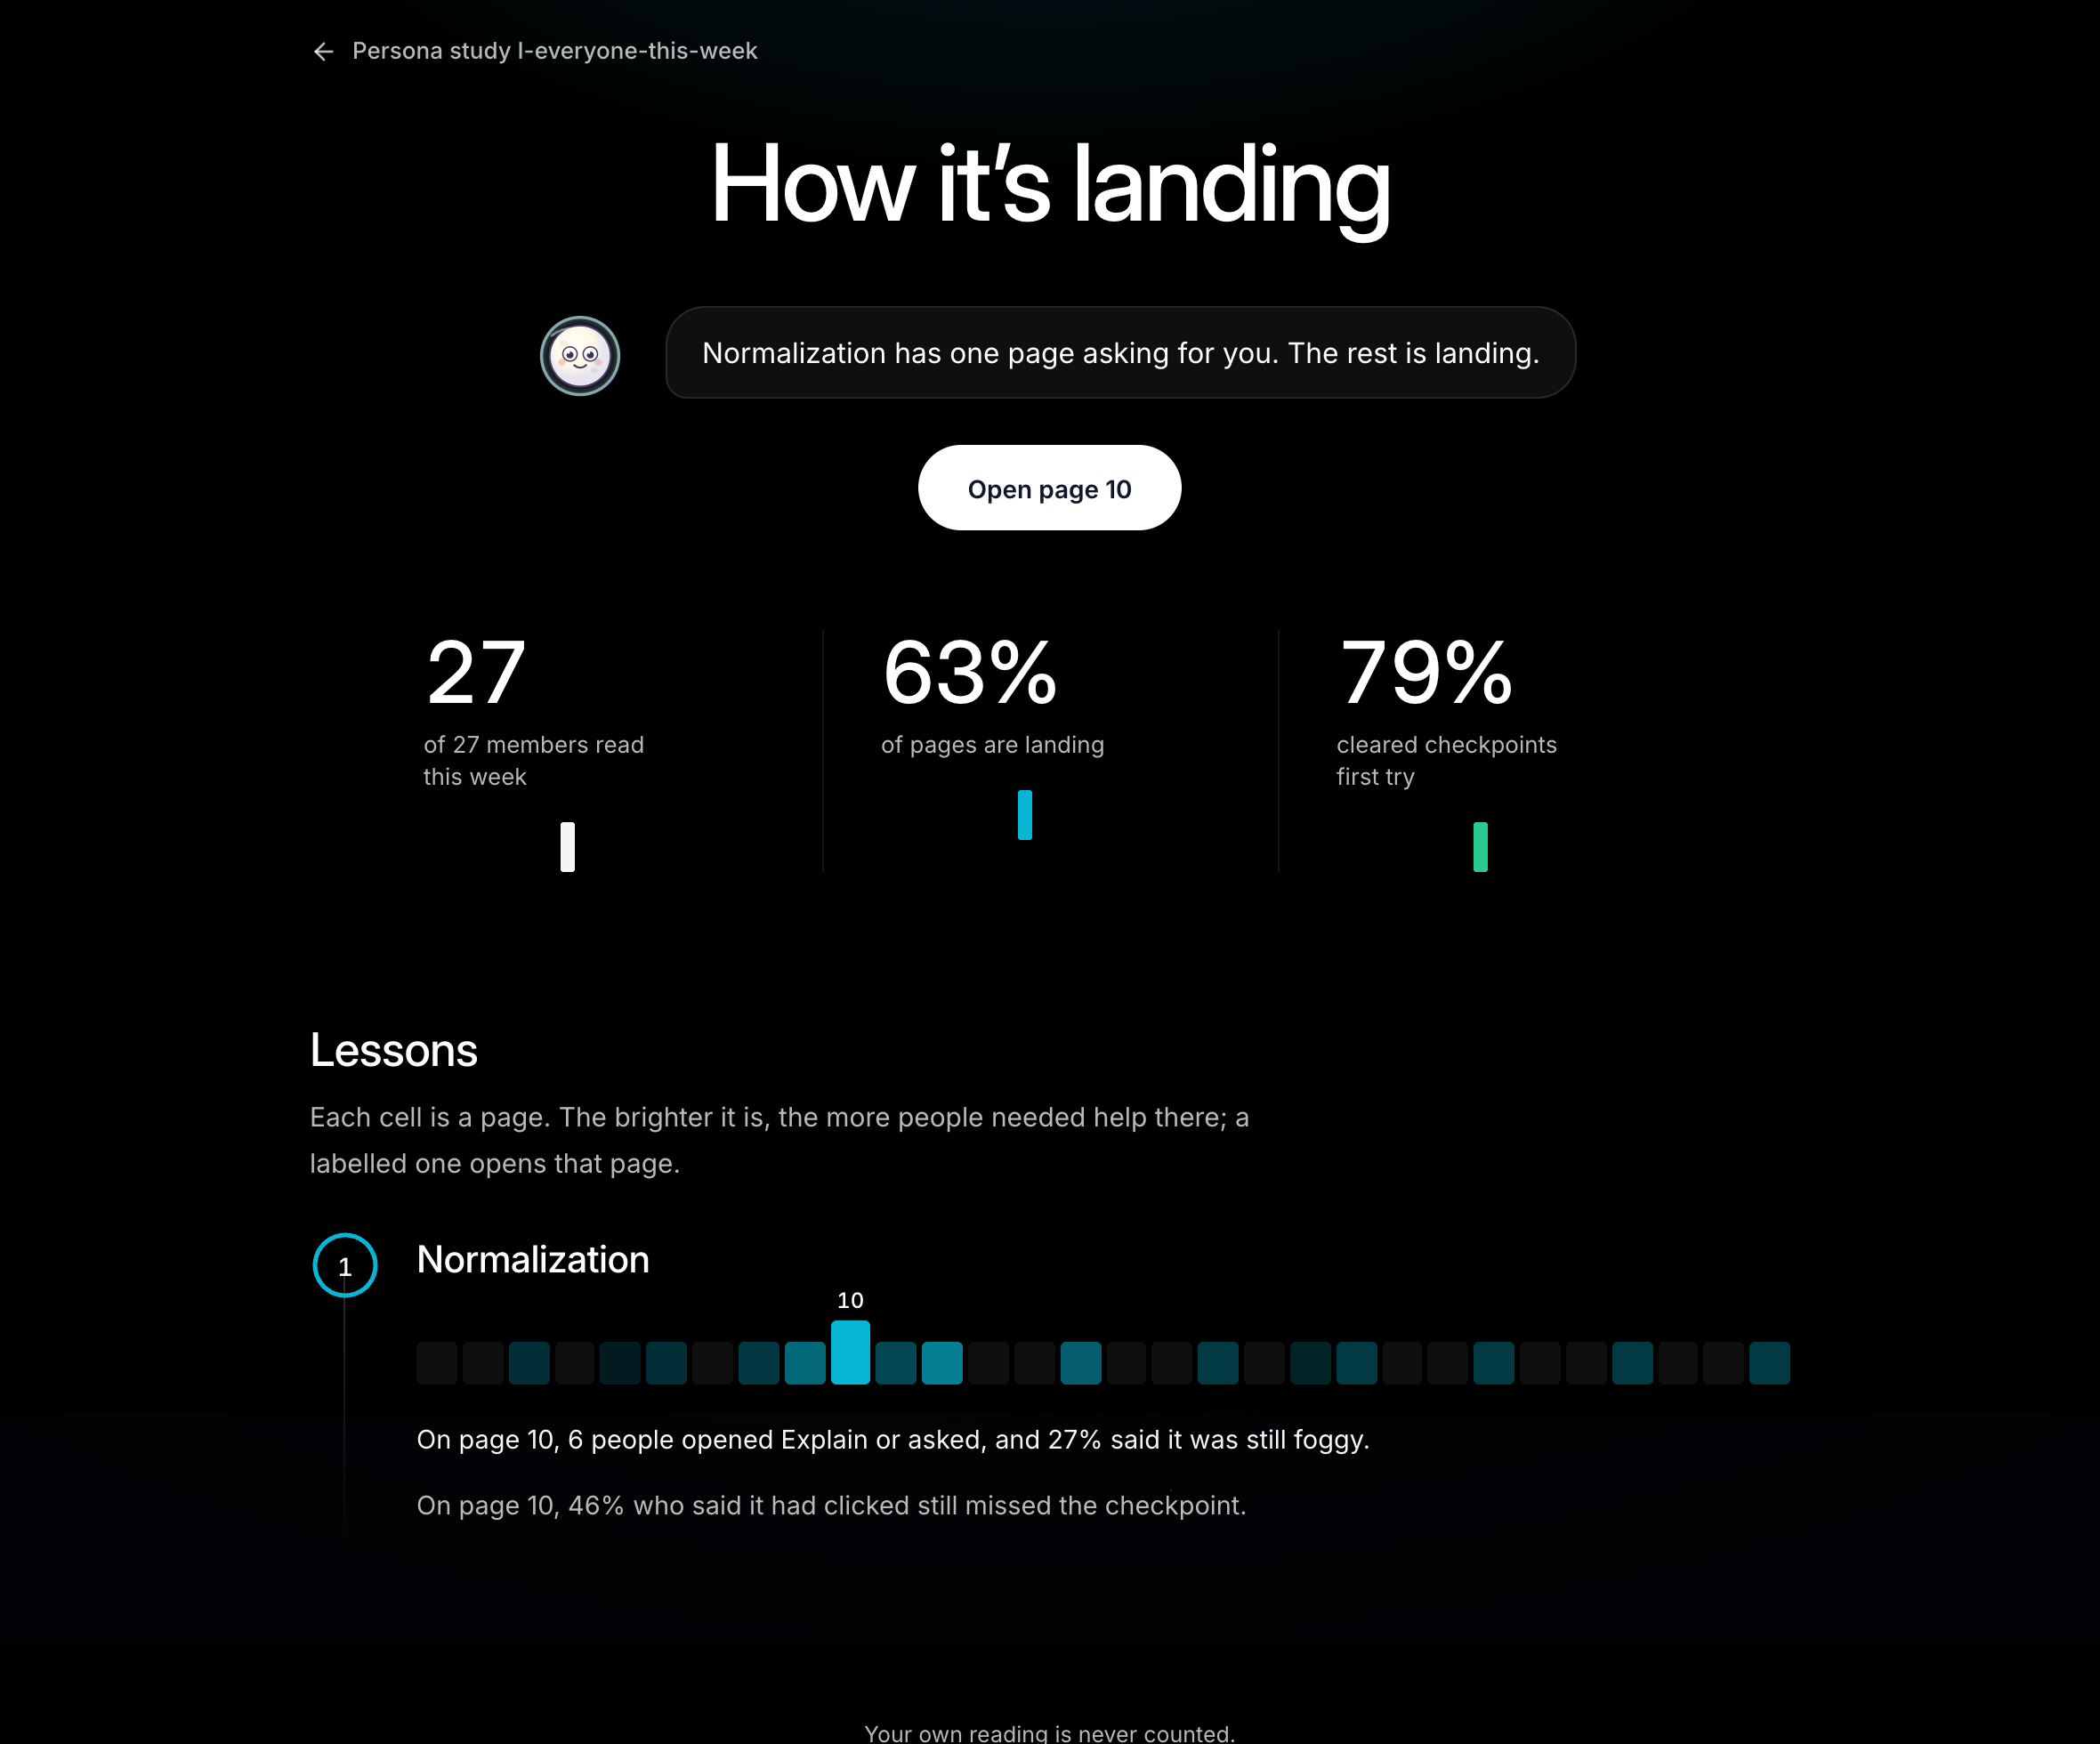
\includegraphics[width=0.85\textwidth]{f21-door-above-floor}
  \caption{The owner's view, drawn by the real screen from the payload of
    arm~I of the study with scripted readers (\cref{sec:c5-evaluation}):
    27~members who all read in the last week. The navigation bar is cropped.}
  \label{fig:door}
\end{figure}

\Cref{fig:door} shows the screen for 27 scripted readers: Luna's sentence
naming the Lesson to look at; the three numbers, each with its last eight
weeks as small bars, where a week without a value stays empty, never zero;
and a map with one cell per page, brighter where more readers reached for
help and a faint outline where fewer than five have read. Each finding stands
below the map as one sentence, for example
\enquote{On page 10, 6 people opened Explain or asked, and 27\,\% said it was
still foggy.} In the last line the owner reads that their own reading is never
counted.

Below the floor the screen shows only Luna's sentence and the last line. For
the control arm of four members the sentence reads \enquote{A few people have
been reading. Patterns show once five people have been through a page.} It
reveals whether anyone has read, not how many.

\section{Privacy by Design}
\label{sec:c5-privacy}

The General Data Protection Regulation asks for data protection by design and
by default~\cite{gdpr2016}. Our system does not anonymise the stored events:
each carries the real user id, and no retention rule is in force. A retention
script exists, but nothing starts it, and it drops old monthly partitions,
which the migrations declare and production lacks
(\code{docs/\allowbreak thesis/\allowbreak evidence/\allowbreak event-table.md}).
The system therefore protects members by limiting what leaves the log.

\begin{description}
  \item[No output about a person.] The owner's view has no list of members, no
    progress per person, and no name. An earlier version showed individuals
    under pseudonyms (PR~\#142). Pseudonymised data remain personal
    data~\cite[Recital~26]{gdpr2016}. In November 2026 we therefore removed
    every person from the view, together with the setting that could switch
    the pseudonyms back on, so that no wrong setting can show individuals
    again (PR~\#175).
  \item[A minimum count per page.] This is the floor of
    \cref{sec:c5-aggregation}. It borrows the minimum group size of
    $k$-anonymity~\cite{sweeney2002kanonymity}, but it is a threshold on
    released numbers, not a property of released records, and only the
    engine's code enforces it.
  \item[Export and erasure.] A user can download their data and delete their
    account, and deleting the account deletes its events.
\end{description}

When a member joins a Space, and on the privacy page, the system promises
\enquote{patterns across at least five people, never by name}
(\code{v4Spaces.json:491}, \code{legal.json:35}). \Cref{sec:c5-findings} shows
that the view keeps this promise by its letter, but not in every sense.

\paragraph{Two paths around the view.}
The view reads the log through the backend, which checks ownership in code
(\cref{sec:architecture}). Two older paths bypass the view, and both were open
in production in November 2026 (\cref{tab:deployed}). The first is a database
policy of the older dashboard. It lets an account with the professor role read
the event rows, with user ids, of every member of a course it owns, the
member's events in other Spaces included and only questions from the reading
view excluded (migration \code{20261027000000}). No screen uses this policy,
and in production only an administrator grants the professor role
(\cref{tab:deployed}).

The second path is a function that every signed-in account may call,
\code{get\_user\_profile}. It returns any user's name, picture, institution,
points, and whether they were active today, whatever the setting that hides a
member's name from other members (migration \code{20260615000200}). By the
policies at the pin an owner may also read who joined their Space, so any
owner could put a name to every member; we read this in the code and did not
test it (migration \code{20260611000000}). \code{get\_user\_profile} is one of
49 functions that run with the rights of the role that defined them, skip
row-level security, and could be called by every signed-in account in
production in November 2026; we did not audit whether each checks its caller
(\cref{tab:deployed}). Migrations that limit the professor policy to the
professor's own Lessons and make the function honour the setting are prepared
but not applied (PRs~\#184 and~\#185).

A third path, the analytics routes of the older interface, let a student who
owned a Space read members' user ids and their questions word for word. One
change limits these routes to professor accounts, with a test over eleven
routes (PR~\#176). Another removed rows per member and questions in members'
own words from what the routes return, which holds even if a check is missing
again (PR~\#175). Production carried the fault until both changes were
deployed in November 2026.

\paragraph{Whom the floor protects against.}
We see three ways around the floor and tried none. \emph{Padding:} the floor counts accounts, and any new
account can join any Space, published or not, through the database interface
and write its own events (migration \code{20260604000000};
\cref{tab:deployed}). Four extra accounts therefore lift a page with one real
reader above the floor. \emph{Differencing:} the view is recomputed over a
moving window of 56~days whenever its five-minute cache has expired, so an
owner who compares the view before and after one known member read a page
learns that member's part. \emph{Homogeneity:} a share of 100\,\% reveals that
every reader reached for help, a value that a minimum group size does not
protect and that $\ell$-diversity
addresses~\cite{machanavajjhala2007ldiversity}. Differential privacy would
bound what one person can change in a released number, also over repeated
releases~\cite{dwork2006dp}; our view adds no noise. The floor therefore
protects against accidental exposure in a small group, not against an owner
who wants to find out about one member.

\section{Evaluation}
\label{sec:c5-evaluation}

\subsection{Method: A Study with Scripted Readers}
\label{sec:c5-method}

We asked a narrower question than RQ2, one that the code can answer: given
readers who behave in known ways, does the owner's view show what it should,
and withhold what it should? A \emph{scripted reader} is a simulated member
whose behaviour we fixed in advance: which pages it reads and for how long,
where it asks, how it checks in, and whether it answers checkpoints right.
Synthetic learner data has been proposed for testing learning-analytics
software without the privacy risks of real data~\cite{berg2016synthetic};
here it also stands in for data that did not arrive. A script builds one Space
with one Lesson of 30~pages, writes the scripted readers' events into the
engine's input, and calls the function that serves the owner's view, with
fixed strings in place of the model that writes themes
(\code{backend/eval/persona\_study.py} at \code{a342dea9}, whose engine is
identical to \code{2e146f51}).

We chose five kinds of scripted reader, the \emph{personas}, and all their
values ourselves, not from data (\cref{sec:c5-personas-detail}). A
\emph{steady} reader reads every page, checks in with \emph{Clicked}, and
clears the checkpoints. A \emph{struggling} reader stays three times as long
on the hard pages 8 to 12, asks there, checks in with \emph{Still foggy} on
page~10, misses that checkpoint, and turns back from page~13. An \emph{asker}
asks on every third page, a \emph{skimmer} spends under five seconds per page
and stops at page~10, and an \emph{overconfident} reader checks in with
\emph{Clicked} everywhere and misses the checkpoint on page~10. Eight
\emph{arms}, each a scripted Space with a fixed mix of personas, make up the
study (\cref{tab:persona}).

Before the first run we wrote down 23 expectations: which findings must appear
in which arm, and which must not. We committed them together with the results,
so only our word, not the commit history, shows that they came first. Two
further arms, added after the result to explain misses, are marked post hoc
and do not count. A \emph{seed} is the start value of the random-number
generator, so each seed gives a different but repeatable draw of reading times
and answers. After the published run, with one seed per arm, we ran every arm
with 100 seeds, under a protocol committed before that run, to see which
results depend on chance (\cref{tab:sweep}).

\subsection{Results}
\label{sec:c5-results}

\begin{table}[htbp]
  \centering
  \small
  \caption{The study with scripted readers, run in November 2026 at \code{2e146f51}: 10
    arms, 5{,}370 events. \enquote{Met} counts expectations written before the
    first run.
    Arms I and J are post hoc. One seed per arm; \cref{tab:sweep} gives 100. Source:
    \code{docs/thesis/experiments/persona-study/RESULTS.md}.}
  \label{tab:persona}
  \begin{tabular}{@{}llp{0.42\textwidth}l@{}}
    \toprule
    Arm & Members & What the owner's view contained & Met \\
    \midrule
    A & 6 struggling, 6 steady & hotspot on page 10, speed bump on page 12; numbers empty & 4 of 5 \\
    B & 3 struggling, 10 steady & hotspot on page 10 & 0 of 2 \\
    C & 5 askers, 5 steady & nothing; no themes & 0 of 1 \\
    D & 4 askers, 6 steady & nothing; no themes & 1 of 1 \\
    E & 8 skimmers, 4 steady & leaky bucket after page 10, pages 1 to 10 skipped & 3 of 3 \\
    F & 6 overconfident, 4 steady & calibration gap on page 10 & 1 of 1 \\
    G & 4 members (control) & nothing: reach \code{few}, all values \code{null} & 9 of 9 \\
    H & 27, all five personas & hotspot and calibration gap on page 10; numbers empty & 0 of 1 \\
    \midrule
    I & the mix of H again, one week & as H; numbers 27, 63\,\%, 79\,\% & post hoc \\
    J & 5 confused askers, 5 steady & hotspot on page 10 with themes from 5 askers & post hoc \\
    \bottomrule
  \end{tabular}
\end{table}

\Cref{tab:persona} gives the published run. The engine met 18 of the 23
expectations, a weak measure on its own, because 15 of them ask the view to
withhold something, nine in the control arm~G. Split by kind, the engine met 5
of the 8 expectations that ask the view to show something and 13 of the 15
that ask it to withhold something; an engine that never reports a finding or a
theme meets 1 and 15 (\code{mute\_engine.py}). Over 100 seeds our engine met
16 to 19 of the 23, with a median of 17 (\cref{tab:sweep}), so the published
run was a good draw.

In arms A, E, and F the planted findings held at every seed. The struggling
readers of arm~A produced a finding on page~10 and a speed bump on page~12,
the skimmers of arm~E a leak and skipped pages, and the overconfident readers
of arm~F a calibration gap. On page~10 of arm~A the finding was the hotspot in
19 seeds and the more specific overpacked page in the other 81; the overpacked
page replaces the hotspot when the page's reading time also runs long. One
finding appeared that no persona was built to cause: in four seeds of arm~C
and one of arm~A, random checkpoint misses produced a calibration gap on a
page other than page~10. In groups this small, chance alone can raise a
finding. In the control arm of four members the payload held no finding, no
theme, and no weekly number at any seed, and the screen showed only the
sentence quoted in \cref{sec:c5-door} and the last line.

Tests without readers fix the same rules: 141 unit tests of the engine and 62
database tests of the event log, its access rules, and erasure, which replay every migration into an empty Postgres and so
test the database that the migrations describe, not production
(\cref{sec:c5-privacy}). No test exercises row-level security through an API
route: the ownership checks in code and the database policies are each
tested, but the place where they meet is not.

\subsection{Three Things the Misses Showed}
\label{sec:c5-findings}

None of the five misses departs from the code's rules. In arms A, C, and H our
expectations had misread the rules. Arm~B's two misses show that the rules do
not keep the promise made to members, that patterns rest on at least five
people.

\paragraph{The numbers cover the current week.}
In arms A and H all three numbers were empty although 12 and 27 members had
read. The view shows the current week, and the scripted readers read on single
days spread over eight weeks, so in neither arm did the current week reach
five readers. Arm~I places the same 27 readers in one week, and the numbers
appear. A Space with fewer than five readers per week shows no numbers even
when the map is full.

\paragraph{The floor counts readers, not the people a finding is about.}
In arm~B three of thirteen members checked in with \emph{Still foggy} on
page~10, and the view reported a hotspot at every seed, because these
check-ins are planted, not random. All thirteen readers of the page checked
in, so it was above the floor, and three of thirteen are 23\,\%, above the
hotspot rule of 20\,\%. The view shows no name and no count of three, so the
promise holds by its letter. It does not hold in the stronger sense that five
people stand behind a pattern: an owner who knows the group may guess who the
three are. With one struggler fewer, two of twelve are 17\,\% and the hotspot
vanishes, so one person can switch a finding on or off. Only the speed bump
counts the people a finding is about. We did not change the engine after the
study, so this remains a limit; the change to make is the stricter rule of
five people behind each finding.

\paragraph{Themes explain a hotspot and nothing else.}
In arm~C five members asked about the same pages, and no themes appeared. The
engine makes themes only for hotspot pages, and these askers checked in with
\emph{Unsure}, which the hotspot rule does not count as \emph{Still foggy}.
What five people ask about a page that is not a hotspot reaches no one.

\subsection{Limits}

The study tests whether the aggregation separates known behaviours and whether
the floor holds. It verifies that the engine implements the rules of
\cref{tab:detectors}; it does not validate that the rules describe real
reading, Boehm's distinction between building the product right and building
the right product~\cite{boehm1984verifying}. Most personas sit far from the
thresholds, but in arm~A the reading time of page~10 sits near the line
between the hotspot and the overpacked page, and the random draw decides
between them. There is one Lesson and one Space. Fixed strings replaced the
model that writes themes, so the study shows nothing about what real themes
might reveal. We wrote both the engine and the study, so expectations and code
can share a misreading. And we did not observe whether an owner changes a page
after seeing a finding, the step that closes the loop.

\section{Answer to RQ2}
\label{sec:c5-answer}

\paragraph{Model.} One log with seventeen checked event types, such as a page
view, a question, or a check-in, records what learners do. A write that fails
drops the event, never the reader's request.

\paragraph{Aggregate.} A pure function turns the last 56~days of a Space's
events into facts per page, from what readers do, say, and get right. Below a
floor of five readers a value is \code{null}, not zero.

\paragraph{Feed back without showing a learner.} The view shows no person and
no finding or share for a page with fewer than five readers, and it never
counts the owner. It falls short of the stricter standard of
\cref{sec:analytics-privacy}: one confused rater among five can carry a
hotspot, padding and differencing get around the floor, and two older paths
stay open until the prepared fixes are applied
(\cref{sec:c5-privacy,sec:c5-findings}).

\paragraph{What the view can tell.} The view shows an owner which page
confuses readers, where they leave, which pages they skip, where they turn
back, and where they feel sure but are wrong. With scripted readers it
reported each of these behaviours at all 100 seeds when the behaviour had an
arm of its own, and for a Space of four it showed no finding, theme, or number. In a mixed group,
a behaviour that few of a page's readers share stays below the rules. The view
shows no weekly numbers in a week with fewer than five readers, and themes
only on a page that is already a hotspot (\cref{sec:c5-findings}). We did not
observe whether real owners use the view to improve their pages.
